\section{Cryptographic Security Analysis}
\label{sec:security_analysis}

The analysis in Section~\ref{sec:noise-errors} demonstrates the protocol's \textit{robustness}, identifying the physical error thresholds at which the teleported charge signal $\langle \Delta Q_B \rangle$ flips sign---a catastrophic failure. However, a full security proof requires a more rigorous, cryptographic framework to guarantee that a positive secret key rate $K$ exists, even in the presence of noise below this threshold. This section outlines this framework, transitioning from protocol-specific attacks to a quantitative security proof against general coherent attacks by an eavesdropper, Eve.

\subsection{Protocol-Specific Attack Models}
\label{sec:attack_models}

As established in \cite{QKDbyQET}, the protocol is inherently secure against several key attack models. In a Man-in-the-Middle (MITM) attack, Eve may know the Hamiltonian, intercept the classical communication (Alice's basis choice $\sigma_A$ and bit $a$), and attempt to forge Bob's result. This attack fails because Bob's outcome (the sign of $\langle \Delta Q_B \rangle$) depends not only on the classical bit $a$ but also on the shared quantum correlations. Eve cannot deterministically reproduce the correct sign without possessing the entangled state, and any attempt to do so would require post-selection capabilities, which are not physically realizable.

In an intercept-resend attack, where Eve establishes separate entangled states with Alice and Bob, the protocol also fails. Bob's measurement outcome will be uncorrelated with Alice's bit, resulting in a random key string that will be detected during parameter estimation.

Furthermore, as noted in Section~\ref{sec:numerical_sim}, the use of a random measurement basis by Alice (e.g., randomly choosing between $\sigma_A = X_0$ and $\sigma_A = Y_0$ for the $H^{(2)}$ model) protects against an adversary performing weak measurements to learn about state imperfections \cite{QKDbyQET}.

\subsection{Quantitative Security and Secret Key Rate}
\label{sec:key_rate_formula}

While robust against these specific attacks, a general security proof must bound the information Eve can gain from any physical interaction, including coherent attacks. The standard approach \cite{Scarani2009} is to compute the asymptotic secret key rate, $K_{\text{asym}}$, (in the limit of infinite signals) which is lower-bounded by the Devetak-Winter formula \cite{Devetak2005}:
\begin{equation}
    K_{\text{asym}} \ge 1 - h(e_{\text{bit}}) - h(e_{\text{ph}})
\end{equation}
where $h(x) = -x \log_2(x) - (1-x) \log_2(1-x)$ is the binary entropy function. Here, $1 - h(e_{\text{bit}})$ bounds the classical mutual information between Alice and Bob, $I(A:B)$, and $h(e_{\text{ph}})$ bounds the Holevo information $\chi(B:E)$, which is the upper bound on the information Eve can gain about Bob's key.

\subsection{Parameter Estimation}
\label{sec:parameter_estimation}

To calculate $K_{\text{asym}}$, Alice and Bob must publicly sacrifice a random subset of their measurement data to estimate two key parameters.

\begin{itemize}
    \item \textbf{$e_{\text{bit}}$ ($Q_{BER}$):} The Quantum Bit Error Rate, or $Q_{BER}$, is the error rate measured in the "key generation" basis (e.g., Alice $\sigma_A=X_0$). This is the observed probability that Bob measures the wrong sign (e.g., a positive charge, logical '0') when Alice intended the opposite (e.g., sent $a=0$, logical '1').

    \item \textbf{$e_{\text{ph}}$ (Phase Error):} The Phase Error Rate is the (unmeasured) error rate in the complementary "test" basis (e.g., Alice $\sigma_A=Y_0$).
\end{itemize}

The phase error rate $e_{\rm ph}$ is not measured directly. Instead, it is estimated by using the rounds where Alice and Bob randomly choose \textbf{different} bases. For example, in the $H^{(2)}$ model, Alice's random choice between $\sigma_A=X_0$ and $\sigma_A=Y_0$ is the mechanism for this. The rounds where they use the "mismatched" bases are sacrificed to test the quantum correlations (e.g., visibility). These correlations provide a verifiable upper bound on $e_{\rm ph}$ through entropic uncertainty relations \cite{Tomamichel2011, Koashi2009}.

% This figure is part of the next subsection, it is here for formatting reasons.
\begin{figure}[htbp]
    \centering
    \subfloat[\( N = 2 \) (Secure)]{
        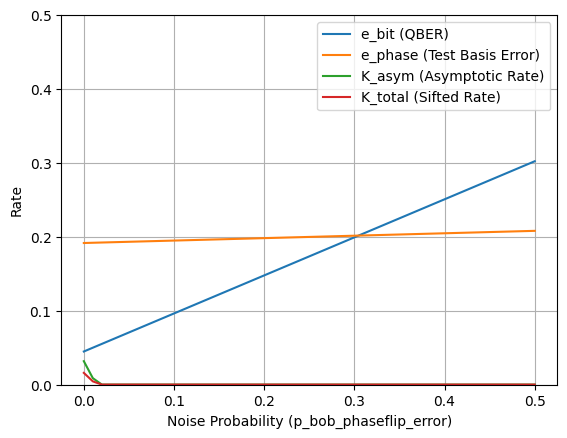
\includegraphics[width=0.32\textwidth]{plots/security/key_rates_vs_bob_phaseflip_J2_h1_N2.png}
        \label{fig:key_rates_n2}
    }
    \hfill
    \subfloat[\( N = 3 \) (Insecure)]{
        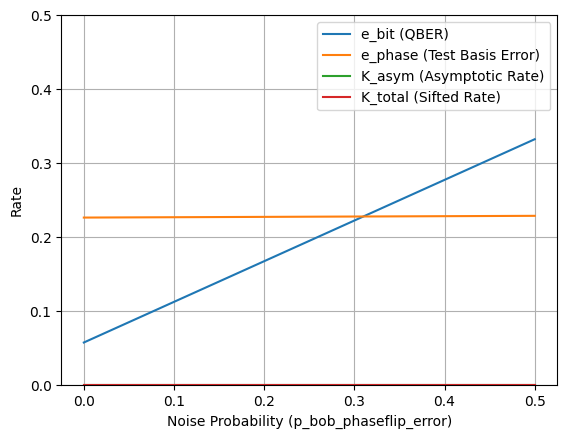
\includegraphics[width=0.32\textwidth]{plots/security/key_rates_vs_bob_phaseflip_J2_h1_N3.png}
        \label{fig:key_rates_n3}
    }
    \hfill
    \subfloat[\( N = 4 \) (Insecure)]{
        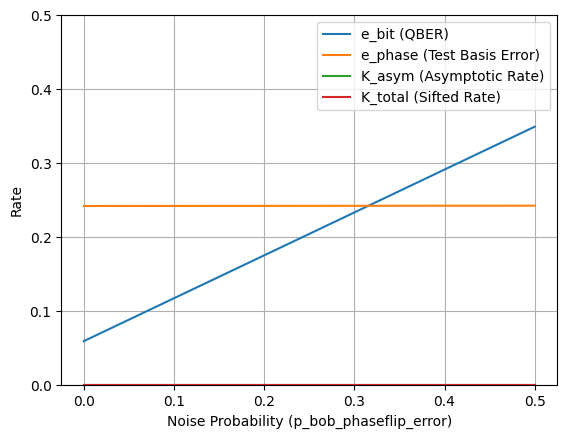
\includegraphics[width=0.32\textwidth]{plots/security/key_rates_vs_bob_phaseflip_J2_h1_N4.png}
        \label{fig:key_rates_n4}
    }

    \caption{Asymptotic key rate analysis for the $H^{(2)}$ model ($J=2, h=1$) under phase-flip noise on Bob's site. Plots show the $Q_{BER}$ ($e_{\text{bit}}$), the test basis error ($e_{\text{ph}}$), and the resulting asymptotic key rate ($K_{\text{asym}}$) as a function of noise probability $p$.}
    \label{fig:key_rates}
\end{figure}

\subsection{Simulation of Key Rate vs. Physical Noise}
\label{sec:simulation_key_rate}

To connect this framework to our physical model, we simulate the protocol under the "phase-flip at Bob's site" noise model ($p_{\text{bob\_phaseflip}}$) for the $H^{(2)}$ Hamiltonian. For each noise probability $p$, we run two parallel simulations to find $e_{\text{bit}}(p)$ and $e_{\text{ph}}(p)$. These error rates are calculated from the simulation as follows:

\begin{itemize}
    \item \textbf{Key Basis ($e_{\text{bit}}$):} We run the simulation in the key basis ($\sigma_A=X_0$). For a given $p$, we calculate the probabilities $P_{+}(p)$ (Bob measures $\Delta Q_B > 0$), $P_{-}(p)$ (Bob measures $\Delta Q_B < 0$), and $P_{0}(p)$ (Bob measures $\Delta Q_B = 0$), given that Alice sent $a=0$ (logical '1'). In this protocol, measurement outcomes of '0' are ambiguous and must be "sifted" (discarded). The final key is built only from the positive and negative outcomes. Due to the protocol's symmetry, an error is registered if Bob measures positive value. The $Q_{BER}$ (blue line) is the error probability normalized by the total probability of a \textbf{non-sifted} (kept) event: $e_{\text{bit}}(p) = P_{+}(p) / (P_{+}(p) + P_{-}(p))$.
    \item \textbf{Test Basis ($e_{\text{ph}}$):} We run a separate simulation in the test basis ($\sigma_A=Y_0$) with the same noise $p$. We calculate the analogous probabilities $P'_{+}(p)$, $P'_{-}(p)$, and $P'_{0}(p)$ for the $\Delta Q_B$ measurement. As with the key basis, the $P'_{0}(p)$ events are sifted out. The test-basis error $e_{\text{test}}(p) = P'_{+}(p) / (P'_{+}(p) + P'_{-}(p))$ (orange line) provides the upper bound for the phase error rate, so we set $e_{\text{ph}}(p) \approx e_{\text{test}}(p)$.
\end{itemize}
The asymptotic key rate $K_{\text{asym}}$ (green line) is then computed directly from these two error rates using $K_{\text{asym}}(p) = \max(0, 1 - h(e_{\text{bit}}(p)) - h(e_{\text{ph}}(p)))$.

The results for $N=2, 3,$ and $4$ (with $J=2, h=1$) are presented in Figure \ref{fig:key_rates}.

The simulation results in Fig. \ref{fig:key_rates} reveal a critical dependence on the system size $N$.
For the minimal chain $N=2$ (Fig. \ref{fig:key_rates_n2}), the protocol is secure. The asymptotic key rate $K_{\text{asym}}$ (green line) is positive for zero noise, $K_{\text{asym}}(p=0) > 0$, indicating a secure channel. This is achieved despite a high intrinsic phase error $e_{\text{ph}}(p=0) \approx 0.19$ because the bit error rate is sufficiently low, $e_{\text{bit}}(p=0) \approx 0.04$. The resulting key rate $K_{\text{asym}}(p=0) = 1 - h(0.04) - h(0.19) \approx 0.05$ is small but positive. The protocol can tolerate noise up to a threshold of $p_{\text{th}} \approx 0.02$, after which $K_{\text{asym}}$ drops to zero.

For longer chains, $N=3$ (Fig. \ref{fig:key_rates_n3}) and $N=4$ (Fig. \ref{fig:key_rates_n4}), the protocol is not secure for these Hamiltonian parameters ($J=2, h=1$). The key rate is zero for all noise levels, $K_{\text{asym}} = 0$. This failure is not a flaw, but a physical result: the intrinsic quantum correlations are too weak. As seen in the $N=3$ plot, the intrinsic phase error $e_{\text{ph}}(p=0) \approx 0.23$ is so high that the combined information leakage $h(e_{\text{bit}}) + h(e_{\text{ph}})$ exceeds 1, making $K_{\text{asym}}$ negative (and thus plotted as zero).

This result demonstrates that while the protocol is a valid proof-of-concept, its practical application requires careful optimization of the Hamiltonian parameters ($J, h$).

\subsection{Finite-Key Effects and Future Work}
\label{sec:finite_key}

The preceding analysis is in the asymptotic limit of infinite signals. For any practical implementation, one must account for the effects of realistic devices and finite statistics \cite{Xu2020, Renner2005}. For any practical implementation with a finite number of signals, $M$, the asymptotic rate $K_{\text{asym}}$ is an overestimation. A composable security proof must be used, which accounts for the statistical fluctuations in the estimation of $e_{\rm bit}$ and $e_{\rm ph}$ from a finite data set. The composable, finite-key security rate $\ell$ is given by more complex bounds \cite{Tomamichel2012, Lim2014}, which introduce correction terms that depend on $1/\sqrt{M}$ and the desired security parameter $\varepsilon_{\text{sec}}$.

Our analysis confirms the fundamental viability of the charge teleportation mechanism for QKD. The next steps involve a) optimizing the Hamiltonian parameters $J$ and $h$ to maximize the intrinsic key rate and secure distance $N$, and b) applying finite-key analysis to the optimized protocol to determine the practical key rates achievable with a realistic number of signals.
